% =============================================================================
% NeurIPS 2026 Workshop variant — exploratory benchmark / artifact paper
% =============================================================================
% Anonymous-submission PDF metadata strip
\ifdefined\pdfsuppressptexinfo\pdfsuppressptexinfo=-1\fi
\ifdefined\pdfinfoomitdate\pdfinfoomitdate=1\fi
\ifdefined\pdftrailerid\pdftrailerid{}\fi

\documentclass{article}

\usepackage[nonatbib]{neurips_2026}
\usepackage[numbers]{natbib}

\usepackage{iftex}
\ifPDFTeX
  \usepackage[utf8]{inputenc}
\fi
\usepackage[T1]{fontenc}
\usepackage{hyperref}
\hypersetup{hidelinks}
\usepackage{url}
\usepackage{booktabs}
\usepackage{amsfonts}
\usepackage{amsmath}
\usepackage{amssymb}
\usepackage{nicefrac}
\usepackage{microtype}
\usepackage{xcolor}
\usepackage{graphicx}
\usepackage{subcaption}
\usepackage{multirow}
\usepackage{enumitem}
\usepackage{tikz}
\usetikzlibrary{positioning, fit, arrows.meta, backgrounds, calc, shadows, shapes.geometric, shapes.misc, decorations.pathreplacing}

\newcommand{\tinker}{\textsc{Tinker}}
\newcommand{\atropos}{\textsc{Atropos}}
\newcommand{\grpo}{\textsc{Grpo}}
\newcommand{\ours}{\textsc{RL-Finetuning Bench}}

\title{RL-Finetuning Bench: An Exploratory Workshop Artifact for GRPO-Style\\
Post-Training Across Libraries, Models, and Backends}

\author{%
  Anonymous Author(s)\\
  Affiliation withheld for blind review\\
  \texttt{anonymous@neurips.cc}%
}

\newcommand{\answerPartial}[1][]{\textcolor{purple}{[Partial] #1}}

\begin{document}
\sloppy
\hbadness=10000
\vbadness=10000
\hfuzz=2pt

\maketitle

% --- Abstract + intro: workshop-tightened ----------------------------------
% =============================================================================
% Abstract — workshop variant. Reframed per GPT-5.5 Pro v5 review section C
% as an ARTIFACT NOTE: artifact card up front, single descriptive claim,
% one negative control, one residualized within-task ablation. No
% benchmark-leaderboard ambition wording.
% Target: <= 200 words.
% =============================================================================
\begin{abstract}
This is an \textbf{exploratory workshop artifact note}, not a benchmark paper.
We present Zero-Variance Fraction (ZVF) summaries, parser scripts, and a
historical manifest. The run-ID census and file-level release inventory
remain unresolved; the collection mixes GRPO, PPO baselines and unexecuted
plans and does not establish coverage of every named library or task.
Raw group traces and checkpoints are not certified for every row.
The historical artifact is associated with
an anonymous repository documented in
Section~\ref{sec:limitations}.

\textbf{Claim hierarchy (descending strength).}
\textit{(i)} ZVF~$=1\Rightarrow$~zero centered reward contrast is mechanical
(Appendix~\ref{sec:appendix:zvf-formalization}).
\textit{(ii)} Later, separate five-seed Qwen3-8B GSM8K evidence reports
$83.3\%$ vs.\ fixed-baseline $82.0\%$ as a one-sample seed-level
$p{=}0.26$ test, not paired-seed or reviewed-record evidence.
\textit{(iii)} The pooled ZVF--last-10 correlation
($r{=}{-}0.769$, $N{=}15$, $p{=}0.0008$) is task-confounded; within
GSM8K only ($N{=}19$), $r{=}{+}0.40$ ($p{=}0.09$).
We report ZVF as a cheap descriptive logging quantity, not as a
predictive failure detector. Frontier-scale and tool-use rows are
single-seed case studies, released for honesty and not as benchmark numbers.
The rest of this artifact note is a candid evidence-grade table and
discussion prompts for the workshop.
\end{abstract}
\paragraph{August 2026 evidence boundary.} This workshop artifact preserves
case-specific rows and does not pool them as an algorithm ranking or a validated
operator policy.

% =============================================================================
% Introduction — workshop variant. Reframed per GPT-5.5 Pro v5 review (sec. C):
% leads with an ARTIFACT CARD and a one-sentence CLAIM HIERARCHY, then
% explicitly disclaims any leaderboard / "first comprehensive" framing.
% Target: <= 0.75 page.
% =============================================================================
\section{Introduction}
\label{sec:intro}

\paragraph{Artifact card.}
This workshop submission is an \textbf{artifact note} accompanying a release
of: \textit{(i)}~one JSON record per Tinker run with configuration, run ID and
per-step mean reward; \textit{(ii)}~per-step Zero-Variance Fraction (ZVF) and
Gradient Utilization (GU) traces for the runs that logged them;
\textit{(iii)}~a per-run manifest (Appendix~\ref{sec:run-manifest}) and a
per-family configuration table (Table~\ref{tab:configs});
\textit{(iv)}~the driver scripts. The release contains no per-group reward
arrays, rollout JSONL, or Tinker model weights (Section~\ref{sec:limitations}). We do
not claim a ``first comprehensive'' GRPO benchmark, a frontier ranking, or a
definitive algorithm comparison.

\paragraph{Claim hierarchy (one sentence).}
The mechanical ZVF-to-centered-reward-contrast identity is theory; the
five-seed Qwen3-8B GSM8K held-out comparison ($+1.3$\,pp, $p{=}0.26$) is a
null result; the pooled ZVF--last-10 correlation ($r{=}{-}0.769$, $N{=}15$)
is a descriptive finding that is task-confounded and changes sign within
GSM8K ($r{=}{+}0.401$, $N{=}19$); everything else (frontier-scale Tinker rows,
tool-use, group-size sweeps) is B-grade when completed at one seed; C denotes
failed, partial or unstarted cells.

\paragraph{Why this is an artifact note rather than a benchmark.}
Reinforcement-learning post-training now drives much of modern language-model
reasoning and alignment~\citep{ouyang2022training,guo2025deepseekr1nature},
but empirical claims are hard to compare:
PPO~\citep{schulman2017proximal}, GRPO~\citep{shao2024deepseekmath}, and
DPO~\citep{rafailov2024direct} are typically reported on different model
families with different framework defaults, different rollout regimes, and
different reward parsers. Rather than declare a winner, we release the
underlying traces and a candid evidence-grade table
(Table~\ref{tab:evidence-grade}) so that downstream readers can re-pool
or stratify as they see fit. The release separates the 5-seed open-stack TRL arm and the 5-seed
Tinker held-out control from the single-seed closed-backend \tinker{} case
studies; the paper describes what those artifacts do and do not support. Discussion prompts for the workshop are
in Section~\ref{sec:conclusion}.


% =============================================================================
\section{Setup (Compact)}
\label{sec:setup}
% =============================================================================

We log step-level group reward statistics for GRPO-style training. The run
manifest (Appendix~\ref{sec:run-manifest}) lists 75 runs in 44 cells:
46 completed GRPO-style LLM runs (8 on TRL via Modal, 38 on the closed
Tinker API), one LLM PPO run (Llama-3.1-8B-Instruct, Modal H100), 15
classic-RL PPO reference runs (CleanRL, Stable Baselines3, Tianshou; 5 seeds
each) on a synthetic math MDP, and 13 failed, partial, or never-started cells.
The main text additionally reports 9 Tinker runs that are not manifest rows
(the 5-seed held-out control and the 4 matched-budget arms;
Table~\ref{tab:configs}). GRPO runs therefore come from two stacks only, TRL
and Tinker; no PufferLib, rl\_games, or d3rlpy run is included. Completed
GRPO cells cover eight model families (Qwen2.5, Qwen3, Qwen3.5, Llama-3.x,
DeepSeek-V3.1, Nemotron, gpt-oss, Kimi-K2) from 0.5B to ${\approx}1$T total
parameters (at most 37B active). Configurations differ by run family; there
is no single headline configuration. Table~\ref{tab:configs} gives the
settings recorded in the per-run JSON files and W\&B run configs. All Tinker
runs use LoRA and Adam ($\beta_1{=}0.9$, $\beta_2{=}0.95$).

\begin{table}[htbp]
\centering\scriptsize
\setlength{\tabcolsep}{3pt}
\caption{Per-family run configurations behind the main-text numbers, as
recorded in the per-run JSON files (\texttt{experiments/tinker-runs/results/},
\texttt{platform\_tinker/reports/final/}) and W\&B run configs. ``P/step'' is
prompts per optimizer step; ``Max tok'' is the training sampler's
generation cap, taken from the W\&B config (matched budget) or from the
committed driver \texttt{world\_class\_experiments.py} (case-study rows;
temperature 0.8). ``n.r.'' means not recorded in the run record.}
\label{tab:configs}
\resizebox{\linewidth}{!}{%
\begin{tabular}{@{}l l l r r r r r l l@{}}
\toprule
Run family & Backend & Model(s) & LoRA $r$ & lr & $G$ & P/step & Steps & Max tok & Seeds \\
\midrule
TRL reference & Modal L4 & Qwen2.5-0.5B & n.r. & n.r. & n.r. & n.r. & 125 & n.r. & 42,123,456,789,1024 \\
Case studies & Tinker & Qwen3-8B, Llama-3.1-8B-Inst & 32 & $3{\times}10^{-5}$ & 8 & 2 & 30 & 512 & 42 \\
Tool-use probes & Tinker & Qwen3-32B, Llama-3.1-8B-Inst & 32 & $3{\times}10^{-5}$ & 8 & 2 & 30 & 512 & 42 \\
Frontier case studies & Tinker & DeepSeek-V3.1, Nemotron-120B, Qwen3-235B & 16 & $10^{-5}$ & 4 & 2 & 20 & 512 & 42 \\
$G$-sweep & Tinker & Qwen3-8B & n.r. & $10^{-5}$ & 2--32 & n.r. & 30 & n.r. & 42 \\
Held-out control & Tinker & Qwen3-8B & 32 & $3{\times}10^{-5}$ & n.r. & n.r. & 50 & n.r. & 42,137,256,512,999 \\
Matched budget & Tinker & Qwen3-8B & 4 & $3{\times}10^{-5}$ & 2 / 16 & 8 & 160 / 20 & 512 & 123,456 \\
\bottomrule
\end{tabular}}
\end{table}

% =============================================================================
\section{Headline Result: ZVF as a Descriptive GRPO Diagnostic}
\label{sec:zvf-analysis}
% =============================================================================

\textbf{Zero-Variance Fraction (ZVF)} at step $t$ is the fraction of prompts
for which all $G$ completions receive identical rewards:
\[
  \mathrm{ZVF}_t = \frac{1}{|\mathcal{P}_t|}\sum_{p \in \mathcal{P}_t}
  \mathbf{1}\bigl[\operatorname{Var}_{c \sim \mathcal{C}(p)}\,r(c) = 0\bigr].
\]
When $\mathrm{ZVF}_t = 1$, every prompt has zero centered reward-contrast
coefficient in this group-standardized runner; this does not assert a zero total
gradient for objectives with KL, auxiliary losses, clipping, or token masking.
\textbf{Gradient Utilization} is $\mathrm{GU}_t = 1 - \mathrm{ZVF}_t$.

\paragraph{Relation to prior work.}
The zero-advantage property of unanimous groups is not new. It follows from
GRPO's group-standardized advantage~\citep{shao2024deepseekmath}, and DAPO's
dynamic sampling~\citep{yu2025dapo} over-samples prompts and discards exactly
the groups whose accuracy is 0 or 1. For binary rewards, ZVF is therefore the
fraction of groups that DAPO would filter. ZVF adds no algorithm. It is the
same quantity logged as a per-step trace in fixed-$G$ runs that do \emph{not}
filter, so that the wasted fraction is visible after the fact. Dr.~GRPO~\citep{tong2025drgrpo}
removes the standard-deviation and length normalizations of the GRPO
objective; it does not change which groups have zero advantage. We use
per-seed reporting rather than rliable-style aggregate
intervals~\citep{agarwal2021deep} because most cells have one seed.

The $N=15$ pool gives $r=-0.769$; the $N=19$ GSM8K cohort is not a subset of
it. In the extended $N=29$ pool, $r=-0.443$ becomes $-0.026$ with task fixed
effects, and its $N=19$ GSM8K subset has $r=+0.401$ (parametric $p=0.088$).
This $+0.401$ is the single within-GSM8K estimate used throughout the paper.
These are descriptive associations between run-level mean ZVF and last-10
training reward, not causal or predictive validation. The per-row cohort
membership and the analysis CSVs behind these values are not in the
repository, so the values cannot currently be regenerated
(Appendix~\ref{sec:stratified-diagnostics}).

\iffalse
\begin{figure}[t]
\centering
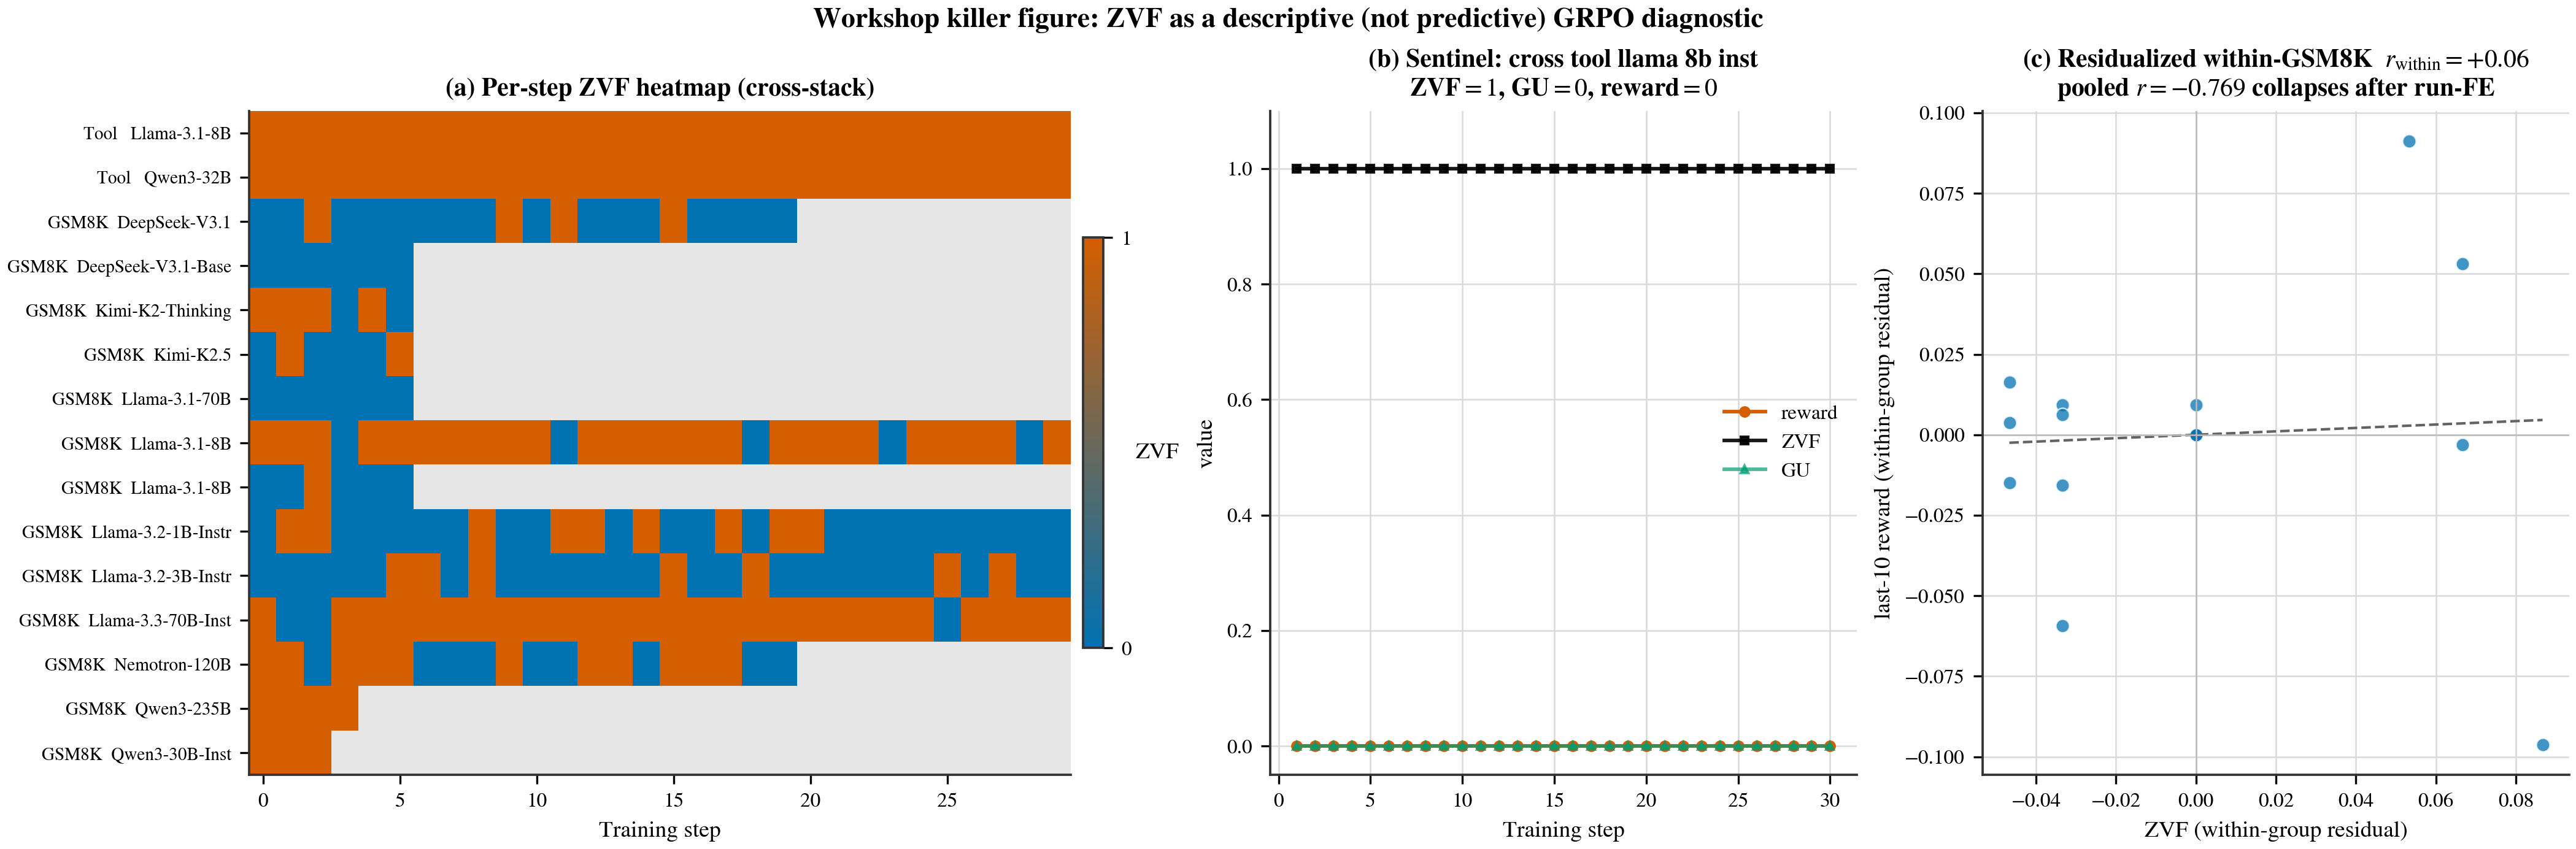
\includegraphics[width=\linewidth]{figures/v2/workshop_killer}
\caption{\textbf{ZVF as a descriptive (not predictive) GRPO diagnostic.}
\textit{(a)}~Per-step ZVF heatmap over the 15 cross-stack runs; red:
$\mathrm{ZVF}{=}1$, blue: $\mathrm{ZVF}{=}0$, grey: no data. Tool-use
rows (top) form the persistent red band that drives the pooled
$r{=}{-}0.769$.
\textit{(b)}~Tool-use sentinel: $\mathrm{ZVF}{=}1$, $\mathrm{GU}{=}0$,
reward$\equiv 0$ at every step.
\textit{(c)}~Residualized within-GSM8K: per-group-demeaned ZVF vs.\
last-10; within-task slope $r_{\mathrm{within}}\approx 0$, in sharp
contrast to pooled $r{=}{-}0.769$.}
\label{fig:workshop-killer}
\end{figure}
\fi

\begin{table}[htbp]
\centering\small
\setlength{\tabcolsep}{5pt}
\caption{Statistical ablation of the ZVF--last-10 correlation under three
sample definitions. The historical $N=15$ pool and $N=19$ subset use different cohorts;
their contrast cannot isolate conditioning. Within-task estimates are descriptive.}
\label{tab:zvf-stat-ablation}
\begin{tabular}{@{}l r r r l@{}}
\toprule
\textbf{Sample} & \textbf{$N$} & \textbf{Pearson $r$} & \textbf{$p$} & \textbf{Note} \\
\midrule
Pooled, cross-stack          & 15 & $-0.769$ & $0.0008$ & B$^{*}$, task-confounded \\
Within-GSM8K (all)           & 19 & $+0.40$  & $0.09$   & extended-pool subset \\
Within-GSM8K (model-varying) &  7 & $+0.13$  & $0.79$   & descriptive \\
\bottomrule
\end{tabular}
\end{table}

\noindent
We do not report bootstrap CIs or permutation $p$-values for the
within-GSM8K rows in this summary table; the full bootstrap analysis and
partial-correlation controls are reported in Appendix~\ref{sec:stratified-diagnostics}.

% =============================================================================
\section{Compact Main Results and Evidence Grade}
\label{sec:main_results}
\label{sec:results}
% =============================================================================

Table~\ref{tab:headline} reports the three kinds of evidence in the release
separately: multi-seed open-stack runs, single-seed Tinker case studies, and
known failure probes. We deliberately do not pool them into one ranking.

\begin{table}[htbp]
\centering\small
\setlength{\tabcolsep}{4pt}
\caption{Headline table, segregated by evidence grade. The open-stack
TRL arm has 5 seeds; the Tinker case studies are single-seed
(cost-constrained, closed backend). For Tinker rows, summaries 1/2 are online
peak/last-10 training reward on the sampled training prompts, under the
512-token generation cap of Table~\ref{tab:configs}. The TRL row reports the
final accuracy per seed (mean 0.734, SD 0.070 over seeds
$\{42,123,456,789,1024\}$; task \texttt{math} on the synthetic \texttt{gen}
split per the run records), not a peak or last-10 value. The Qwen3-235B run is
partial (15 of 20 steps; only 4 step rewards were logged) and is listed
separately.}
\label{tab:headline}
\begin{tabular}{@{}l l l r r r@{}}
\toprule
\textbf{Algo / stack} & \textbf{Model} & \textbf{Task} & \textbf{Seeds} & \textbf{Summary 1} & \textbf{Summary 2} \\
\midrule
\multicolumn{6}{l}{\textit{Multi-seed open-stack}} \\
\midrule
TRL-GRPO (Modal L4) & Qwen2.5-0.5B & math (gen) & 5 & range 0.62--0.81 & mean 0.734 \\
\midrule
\multicolumn{6}{l}{\textit{Single-seed Tinker case studies (\dag closed backend)}} \\
\midrule
GRPO\,\dag        & Qwen3-8B            & GSM8K     & 1 & 62.5\% & 34.4\% \\
GRPO\,\dag        & Llama-3.1-8B-Inst   & GSM8K     & 1 & 100\%  & 84.4\% \\
GRPO\,\dag        & DeepSeek-V3.1       & GSM8K     & 1 & 100\%  & 85.0\% \\
GRPO\,\dag        & Nemotron-120B       & GSM8K     & 1 & 87.5\% & 16.2\% \\
\midrule
\multicolumn{6}{l}{\textit{Partial run and failure probes (not benchmark numbers)}} \\
\midrule
GRPO\,\dag        & Qwen3-235B-A22B     & GSM8K (partial) & 1 & 100\% & --- \\
GRPO\,\dag        & Qwen3-32B           & Tool-use  & 1 & 0\%    & 0\%    \\
GRPO\,\dag        & Llama-3.1-8B-Inst   & Tool-use  & 1 & 0\%    & 0\%    \\
\bottomrule
\end{tabular}
\end{table}

\paragraph{Held-out negative control.}
Five Qwen3-8B GRPO runs on Tinker (LoRA rank 32, lr $3{\times}10^{-5}$, 50
steps, seeds $\{42,137,256,512,999\}$; Table~\ref{tab:configs}) were each
evaluated greedily (max 2{,}048 new tokens) on the first 200 GSM8K test
problems. The base model scores $82.0\%$ under the same protocol. Per-seed GRPO
accuracy is $83.0, 82.5, 80.5, 84.0, 86.5\%$ (mean $83.3\%$). The seed-level
difference is $+1.3$\,pp (95\% $t$ interval $[-1.4,+4.0]$\,pp; one-sample
$t_4{=}1.32$, $p{=}0.26$ against the single deterministic base score). The
paired per-prompt McNemar test is non-significant for every seed (exact
$p\in[0.09,1.00]$). A majority vote over the five seeds reaches $87.5\%$
(McNemar exact $p{=}0.035$); this ensemble comparison was chosen post hoc and
is not a single-model result. The supported statement is a null: online
training reward does not by itself imply held-out gain. These runs are not
manifest rows; their records are \texttt{platform\_tinker/reports/final/gsm8k\_heldout\_seed*.json}
and W\&B project \texttt{tinker-rl-scaling}.

\paragraph{Training reward is not held-out accuracy.}
The Qwen3-8B case study reaches only $34.4\%$ last-10 training reward
(the five held-out-control runs: $27.5$--$35.0\%$), far below the same model's
$82.0\%$ held-out base accuracy. The two measurements differ in protocol. The
case-study run samples at temperature 0.8 with a 512-token cap, and its
training prompt is a raw ChatML string that does not disable Qwen3's thinking
mode; the training cap of the held-out-control runs is not recorded.
Evaluation is greedy with a 2{,}048-token cap.
The case-study run did not log completion lengths. The four matched-budget
Qwen3-8B arms, which use the same 512-token cap, did: in both $G{=}16$ arms the
mean completion length is $\ge508.6$ tokens at every step, so nearly every
sample is cut at the cap. A post-hoc re-evaluation on the first 200 GSM8K test
items (greedy) confirms the truncation reading. With the case-study prompt,
thinking mode on and a 512-token cap, the base model scores $27.0\%$
(95\% CI $[21.3, 33.5]$) with $100\%$ of generations truncated, close to the
training reward; with thinking disabled and a 4{,}096-token cap it scores
$97.5\%$ with no truncation. The case-study adapter scores $31.0\%$ and
$96.5\%$ under the same two conditions, indistinguishable from base (paired
McNemar $p\ge0.32$)
(\nolinkurl{experiments/results/review_2026-10-18/qwen3_8b_truncation_eval/}).
The low training reward is therefore a truncation effect, not a measure of
GSM8K ability.

\paragraph{Group size: brief.}
We ran a single-seed exploratory $G$-sweep on Qwen3-8B/GSM8K whose results
are non-monotonic across $G$ (last-10 training reward $0.35, 0.29, 0.33, 0.39$
at $G{=}2,4,16,32$). \textbf{We do not headline a winning $G$.} The
token-budget table in Appendix~\ref{sec:appendix:group-size-reconcile} is a
hand-entered illustrative table (\texttt{FALLBACK\_ROWS} in
\texttt{group\_size\_token\_normalized.py}), not measured runs, and cannot
establish an optimal group size. A separate two-seed matched-budget panel on
Tinker (Qwen3-8B, LoRA rank 4, 8 prompts per step, 2{,}560 rollouts per arm;
$G{=}2\times160$ vs.\ $G{=}16\times20$ steps; seeds 123 and 456; W\&B project
\texttt{zvf-training}) adds one trajectory-level datum. The $G{=}2$ arms
reach last-10 training reward $0.90$ and $0.96$ and end in an all-correct
zero-variance regime (last-10 ZVF $0.975$ in both). The $G{=}16$ arms end at
$0.32$ and $0.39$ with last-10 ZVF $0.15$ and $0.10$, with completions at the
512-token cap throughout. Small $G$ trades early step count for endgame
signal exhaustion in this panel; two seeds per arm support no stronger claim.

\begin{table}[htbp]
\centering\small
\setlength{\tabcolsep}{4pt}
\caption{Evidence labels follow the run manifest: A = completed cells with
at least three seeds, B = completed single-seed cells, C = failed/partial
cells. ``Theory'', ``descriptive'' and ``illustrative'' mark claims outside the
A/B/C completion tiers. A seed count alone does not license inference.}
\label{tab:evidence-grade}
\begin{tabular}{@{}p{0.50\linewidth} l p{0.32\linewidth}@{}}
\toprule
\textbf{Claim} & \textbf{Grade} & \textbf{Notes} \\
\midrule
ZVF $\to$ zero centered reward contrast is mechanical & theory & App.~\ref{sec:appendix:zvf-formalization}. \\
ZVF--last-10 $r{=}-0.769$ ($N{=}15$, pooled) & descriptive & Task-confounded; within GSM8K $r{=}+0.401$ ($N{=}19$). \\
Qwen3-8B GSM8K held-out $83.3\%$ vs.\ base $82.0\%$ (null) & A & 5 Tinker seeds, 200 test problems; $p{=}0.26$; paired McNemar n.s.\ per seed. \\
Group-size sweep is non-monotonic; no headline winner & B & single-seed per $G$. \\
Matched-budget $G{=}2$ endgame ZVF wall & descriptive & 2 seeds/arm; 512-tok cap. \\
Token-budget table, accuracy argmax $G{\approx}32$ at $T{\ge}16$M & illustrative & hand-entered table, no runs; not an optimum. \\
Frontier-scale Tinker case studies & B & single-seed, closed backend. \\
Tool-use $0\%$ reward across runs & B & task-design failure, not capability. \\
\bottomrule
\end{tabular}
\end{table}

% =============================================================================
\section{Reproducibility and Limitations}
\label{sec:limitations}
% =============================================================================

\paragraph{What the artifact contains.}
The artifact repository (anonymous mirror:
\url{https://anonymous.4open.science/r/agentic-grpo-bench-anon-2C6B})
holds the driver scripts and one JSON record per Tinker run
(\texttt{experiments/tinker-runs/results/}) with configuration, run ID,
per-step mean reward, and, where logged, per-step ZVF and GU. The TRL and
classic-RL rows have summary records only (\texttt{master\_results.csv}).
The artifact contains \emph{no} per-group or per-completion reward arrays
and no rollout JSONL, so ZVF cannot be recomputed from raw rewards, and
stratified analyses needing per-group data cannot be run from it. Tinker
model weights are not released; the per-run Hugging Face repositories hold
only a model card and the results JSON. The run counts in
Section~\ref{sec:setup} are counts of manifest rows; the manifest is not an
immutable run-ID census.

The release has known gaps that the workshop framing makes explicit. (i)~Most
Tinker experiments are single-seed and depend on a closed-source backend; we
report them descriptively. (ii)~Empirical evidence concentrates on
short-horizon GSM8K with binary verifiable rewards; tool-use, code, and
non-math coverage are sparser and yield negative or descriptive evidence
only. (iii)~Train-set reward in the Tinker case studies is \emph{descriptive
instrumentation}, not an inferential signal, and under the 512-token cap it
largely reflects truncation (Section~\ref{sec:results}). The only inferential
result is the held-out null ($83.3\%$ vs.\ $82.0\%$, $p{=}0.26$, 5 seeds).
Tinker-derived stratified correlations (e.g., the within-GSM8K ZVF
re-analysis) are reported as artifact analyses with closed-backend caveats,
not as benchmark statistics. (iv)~Cross-library comparisons are confounded by
checkpoint, hardware, and default-config differences; we report them as
stack-level observations, not as algorithm-level statements. (v)~Direct KL
tracking was blocked by a PyTorch gradient-graph error; the corrected
implementation is in the artifact but is not validated against ZVF in the
current paper. (vi)~Verifiable rewards reduce reward-model subjectivity but
do not eliminate reward hacking, format gaming, or train-set reward
inflation; we do not claim they do.

% =============================================================================
% =============================================================================
% Conclusion — workshop variant. Reframed per GPT-5.5 Pro v5 review (sec. C
% Move D): replaces vague open-question prose with 3-5 SHARP, CONCRETE
% workshop questions that reviewers/attendees could discuss.
% Target: <= 0.5 page.
% =============================================================================
\section{Discussion and Concrete Workshop Questions}
\label{sec:conclusion}

The workshop release is deliberately exploratory. Its strongest evidence is
short-horizon GSM8K dynamics; non-math coverage is a stress case, not a
result. We treat ZVF as a cheap descriptive diagnostic, not a predictive
failure detector. The later Qwen3-8B comparison reports a small,
non-significant difference against a fixed base; it is separate future-paper
evidence, not a reviewed-record held-out control.

\paragraph{Five concrete questions for the workshop.}
We invite attendees to engage with five specific, testable questions raised
by this release rather than open-ended philosophizing:
\begin{enumerate}[leftmargin=1.4em,topsep=2pt,itemsep=2pt]
  \item Does step-level ZVF predict reward change \emph{within} a single
        run, controlling for run fixed effects, on stacks beyond Tinker?
        Our residualized within-GSM8K scatter
        (Figure~\ref{fig:workshop-killer}c) finds $r_{\mathrm{within}}$
        close to zero; is this a backend artifact or a general property?
  \item Under a fixed rollout-token budget, where does group size trade early
        step count for endgame contrast? Our two-seed $G{=}2\times160$ versus
        $G{=}16\times20$ panel ends with the small-$G$ arms at an all-correct
        ZVF wall while $G{=}16$ remains mid-learning; a separate 3-seed
        reanalysis places a fitted apex near $G{\approx}32$ for one stack and
        budget. Neither identifies a universal optimum. The needed experiment
        is a directly trained, multi-seed, token-matched sweep on open stacks.
  \item Are there tasks where high-ZVF cells \emph{do} predict downstream
        collapse, beyond GSM8K? Tool-use is a degenerate $\mathrm{ZVF}{=}1$
        case from step 1; the genuinely interesting test is on
        intermediate-density tasks (MATH-500 at low temperature, code
        with partial-credit rewards).
  \item What minimum disclosure makes a managed-API result count as
        benchmark evidence? Our Tinker rows are reproducible only at the
        level of API call scripts; should the community require GRPO
        loss / reward normalization / hardware metadata for a managed-API
        row to count as anything beyond a case study?
  \item Should ZVF-style diagnostic claims require raw per-group rollout
        JSONL by default? Our release bundles step-level aggregates for
        every run but raw JSONL only for a documented subset; we invite
        the workshop to align on a minimum raw-artifact bar.
\end{enumerate}


% Ethics, Limitations, and Broader Impact (P8-specific; the shared
% ethics_statement_zvf.tex describes content that P8 does not contain)
% =============================================================================
% Ethics, limitations, and broader impact --- P8 workshop note only.
% Replaces the shared ethics_statement_zvf.tex for P8, which describes
% datasets, libraries, releases and results that P8 does not contain.
% =============================================================================
\section{Ethics, Limitations, and Broader Impact}
\label{sec:impact_standalone}

\paragraph{Dual use.}
The release consists of GRPO driver scripts for GSM8K~\cite{cobbe2021training}
and a ten-prompt synthetic tool-call task, per-run JSON records, and logging
code for ZVF. No Tinker model weights are released. The held-out
comparison in Section~\ref{sec:results} is a null result, so the release does
not demonstrate a capability gain. Public GRPO implementations of at least
equal capability already exist~\cite{shao2024deepseekmath,vonwerra2022trl}.
GRPO optimizes a proxy reward and can reward-hack~\cite{skalse2022specificationgaming};
ZVF measures within-group reward contrast and does not detect reward hacking.

\paragraph{Data.}
GSM8K (MIT licence; 7{,}473 train / 1{,}319 test problems) is used unmodified.
Training samples the train split; the held-out evaluation uses the first 200
test problems. The tool-use probes use ten prompts over five invented tools
(calculator, weather, search, reminder, translate) written by the authors and
contained in the driver script. The classic-RL PPO reference runs use a
synthetic math environment. No web scraping, human subjects, or personal data
are involved.

\paragraph{Compute.}
We did not retain billing exports or GPU-hour telemetry, so we report no
itemised spend. We give no carbon estimate for the Tinker runs: the hardware and its utilization are not disclosed, and the
client wall-clock time includes queueing and API stalls.

\paragraph{Closed backend.}
Most rows depend on the managed Tinker API. Our driver computes advantages
(group mean and standard deviation) and the policy-gradient loss on the client
through \texttt{forward\_backward\_custom}, so those are auditable. Sampler and
trainer numerics, hardware, and scheduling are not. Tinker rows are case
studies; replication requires Tinker access.

\paragraph{Methodological limits.}
Tinker training horizons are short (20--50 steps; 160 for the $G{=}2$ matched-budget
arms). Most Tinker cells have one seed. All Tinker runs use LoRA. Tinker
training reward is measured on sampled training prompts (under a 512-token cap
in the case studies) and is not a measure of GSM8K accuracy (Section~\ref{sec:results}). The study is
exploratory and not pre-registered; reported $p$-values are not corrected for
multiple comparisons.


\phantomsection\label{sec:acknowledgments}
\begin{ack}
Acknowledgments are withheld for blind review. We thank the Tinker team for
API access, the Modal team for GPU compute credits (H100 cluster), Weights
\& Biases for experiment tracking infrastructure, and Hugging Face for model
hosting. We are grateful to the open-source communities behind TRL, Stable
Baselines3, CleanRL, Tianshou, and the broader Hugging Face ecosystem.
\end{ack}

\bibliographystyle{plainnat}
\bibliography{../references}

% =============================================================================
\appendix
% =============================================================================
% Workshop appendix: full benchmark design, run manifest, ZVF formalization,
% group-size token-budget reanalysis, and pipeline spec. NOTE: workshop
% submission does NOT include the NeurIPS Paper Checklist (workshops do not
% require it).
% =============================================================================

% =============================================================================
% Run manifest appendix --- review-driven addition
% Compiled from experiments/master_results.csv and the per-run JSONs in
% experiments/tinker-runs/results/ at submission time. The campaign_v2 batch
% (campaign_v2_20260419_111623.json) supplies the ``Bitter Lesson Campaign''
% rows; the wave2-groupsize subset of that batch supplies the explicit
% group-size ablation rows; wave6_ablations.json supplies the Qwen3-8B
% temperature/rank/batch sensitivity ablation. The ``steps_completed=0''
% entries in master\_results.csv for several scale\_/arch\_/frontier\_ runs
% are stale CSV cells; the per-run JSONs and reward\_trace arrays show those
% runs actually completed (steps and last-10 metrics in the JSONs match
% the values in Table~4 of the DNB variant and the case-study lists in the
% ZVF and workshop variants). This manifest reflects the JSON ground truth.
% =============================================================================
\section{Run Manifest}
\label{sec:run-manifest}

This historical manifest records cells, not a reconciled corpus census.
Its displayed run counts total 75, whereas earlier summaries said 79; no missing
run identities are inferred. Tier A denotes completed multi-seed cells (at least
three independent seeds at fixed configuration), B completed descriptive
single-seed cells, and C failed, partial or unstarted cells. These labels do
not by themselves authorize inference: task, endpoint and independence must
also be verified. Backend access is a separate field. Configuration sweeps
are not seed replication. Artifact checks are historical availability claims,
not a certification that every current output is independently reproducible.

\begin{table}[h]
\centering\scriptsize
\setlength{\tabcolsep}{3pt}
\resizebox{\linewidth}{!}{%
\begin{tabular}{lllllrrrcccc}
\toprule
Tier & Backend & Model & Task & Split & N & Seeds & Steps$_{\max}$ & Reward & Held-out & Logs & Ckpt \\
\midrule
\multicolumn{12}{l}{\textit{Tier A --- multi-seed completed cells, replication metadata; inference requires eligibility}} \\
\midrule
A & Modal       & cleanrl-ppo               & math                & gen     & 5 & 5 & 97280  & BV & --- & \checkmark & --- \\
A & Modal       & sb3-ppo                   & math                & gen     & 5 & 5 & 100352 & BV & --- & \checkmark & --- \\
A & Modal       & tianshou-ppo              & math                & gen     & 5 & 5 & 100000 & BV & --- & \checkmark & --- \\
A & Modal L4    & qwen2.5-0.5b              & math                & gen     & 5 & 5 & 125    & BV & --- & \checkmark & \checkmark \\
B & Tinker      & qwen3-8b (Wave-6: 12 configurations)& gsm8k               & train+held-out & 12 & 1 & 30 & BV & \checkmark & \checkmark & --- \\
A & Tinker      & llama-3.3-70b-inst        & gsm8k               & train   & 4 & 4 & 30     & BV & --- & \checkmark & --- \\
\midrule
\multicolumn{12}{l}{\textit{Tier B --- single-seed completed Tinker case studies}} \\
\midrule
B$^\dagger$ & Tinker      & qwen3-8b (G=8, base)      & gsm8k               & train+held-out & 1 & 1 & 30 & BV & \checkmark & \checkmark & --- \\
B$^\dagger$ & Tinker      & qwen3.5-4b                & gsm8k               & train   & 1 & 1 & 30 & BV & --- & \checkmark & --- \\
B$^\dagger$ & Tinker      & llama-8b-inst (gsm8k)     & gsm8k               & train   & 1 & 1 & 30 & BV & --- & \checkmark & --- \\
B$^\dagger$ & Tinker      & deepseek-v3.1             & gsm8k               & train   & 1 & 1 & 20 & BV & --- & \checkmark & --- \\
B$^\dagger$ & Tinker      & nemotron-120b             & gsm8k               & train   & 1 & 1 & 20 & BV & --- & \checkmark & --- \\
B$^\dagger$ & Tinker      & gpt-oss-20b               & gsm8k               & train   & 1 & 1 & 30 & BV & --- & \checkmark & --- \\
B$^\dagger$ & Tinker      & kimi-k2                   & gsm8k               & train   & 1 & 1 & 20 & BV & --- & \checkmark & --- \\
B & Modal H100  & llama-3.2-3b-inst         & gsm8k               & train   & 1 & 1 & 30 & BV & --- & \checkmark & --- \\
B & Modal H100  & llama-3.2-1b-inst         & gsm8k               & train   & 1 & 1 & 30 & BV & --- & \checkmark & --- \\
B & Modal H100  & qwen3-8b (TRL ref)        & gsm8k               & train   & 1 & 1 & 30 & BV & --- & \checkmark & --- \\
B & Modal H100  & llama-8b-inst             & gsm8k               & train   & 1 & 1 & 30 & BV & --- & \checkmark & --- \\
B & Tinker      & llama-8b-inst (tool)      & tool\_use           & train   & 1 & 1 & 30 & SH & --- & \checkmark & --- \\
B & Tinker      & qwen3-32b (tool)          & tool\_use           & train   & 1 & 1 & 30 & SH & --- & \checkmark & --- \\
\midrule
\multicolumn{12}{l}{\textit{Tier B --- Bitter Lesson Campaign (single-seed Tinker frontier runs, GSM8K, 30 steps, completed)}} \\
\midrule
B & Tinker      & qwen3-8b-base             & gsm8k               & train   & 1 & 1 & 30 & BV & --- & \checkmark & --- \\
B & Tinker      & kimi-k2-thinking          & gsm8k               & train   & 1 & 1 & 30 & BV & --- & \checkmark & --- \\
B & Tinker      & kimi-k2.5                 & gsm8k               & train   & 1 & 1 & 30 & BV & --- & \checkmark & --- \\
B & Tinker      & gpt-oss-120b              & gsm8k               & train   & 1 & 1 & 30 & BV & --- & \checkmark & --- \\
B & Tinker      & qwen3.5-397b              & gsm8k               & train   & 1 & 1 & 30 & BV & --- & \checkmark & --- \\
B & Tinker      & llama-3.1-70b             & gsm8k               & train   & 1 & 1 & 30 & BV & --- & \checkmark & --- \\
B & Tinker      & deepseek-v3.1-base        & gsm8k               & train   & 1 & 1 & 30 & BV & --- & \checkmark & --- \\
B & Tinker      & llama-3.1-8b              & gsm8k               & train   & 1 & 1 & 30 & BV & --- & \checkmark & --- \\
\midrule
\multicolumn{12}{l}{\textit{Tier B --- Group-Size Ablation (Qwen3-8B, GSM8K, single-seed per G, 30 steps, completed)}} \\
\midrule
B & Tinker      & qwen3-8b (G=2)            & gsm8k               & train   & 1 & 1 & 30 & BV & --- & \checkmark & --- \\
B & Tinker      & qwen3-8b (G=4)            & gsm8k               & train   & 1 & 1 & 30 & BV & --- & \checkmark & --- \\
B & Tinker      & qwen3-8b (G=8)            & gsm8k               & train   & 1 & 1 & 30 & BV & --- & \checkmark & --- \\
B & Tinker      & qwen3-8b (G=16)           & gsm8k               & train   & 1 & 1 & 30 & BV & --- & \checkmark & --- \\
B$^\dagger$ & Tinker      & qwen3-8b (G=32) & gsm8k               & train   & 1 & 1 & 30 & BV & --- & \checkmark & --- \\
C$^\S$ & ---         & qwen3-8b (G=64)$^\S$      & gsm8k (extrap.)     & ---     & 0 & 0 & 0  & --- & --- & --- & --- \\
\midrule
\multicolumn{12}{l}{\textit{Tier C --- failed, partial, or never-started cells (listed for honesty)}} \\
\midrule
C & External    & 0.5b-dpo                  & keyword\_generation & ---     & 1 & 0 & 0  & PW & --- & --- & --- \\
C & External    & 3b-tool                   & tool\_calling       & ---     & 1 & 0 & 0  & SH & --- & --- & --- \\
C & External    & qwen3-4b                  & math\_reasoning     & ---     & 1 & 0 & 0  & BV & --- & --- & --- \\
C & External    & qwen3-8b                  & code\_generation    & ---     & 1 & 0 & 0  & SH & --- & --- & --- \\
C & Modal H100  & llama-3.2-1b              & gsm8k (alt run)     & ---     & 1 & 0 & 0  & BV & --- & --- & --- \\
C & Modal H100  & llama-3.2-3b              & gsm8k (alt run)     & ---     & 1 & 0 & 0  & BV & --- & --- & --- \\
C & Modal H100  & qwen3-8b                  & humaneval           & ---     & 1 & 1 & 0  & BV & --- & --- & --- \\
C & Modal H100  & qwen3-8b                  & kl\_tracking        & ---     & 1 & 1 & 0  & ---& --- & --- & --- \\
C & Tinker      & qwen3-235b-moe            & gsm8k (partial)     & train   & 1 & 1 & 15 & BV & --- & \checkmark & --- \\
C & Tinker      & qwen3-30b-moe             & gsm8k (partial)     & train   & 1 & 1 & 20 & BV & --- & \checkmark & --- \\
C & Tinker      & qwen3-30b-moe-inst        & gsm8k (partial)     & train   & 1 & 1 & 10 & BV & --- & \checkmark & --- \\
C & Tinker      & qwen3-32b                 & gsm8k (partial)     & train   & 1 & 1 & 10 & BV & --- & \checkmark & --- \\
C & Tinker      & qwen3.5-27b               & gsm8k (partial)     & train   & 1 & 1 & 10 & BV & --- & \checkmark & --- \\
\bottomrule
\end{tabular}
}
\caption{Per-(backend, model, task) run manifest at submission time.
Tier classification: \textbf{A}~at least three independent seeds at fixed
configuration, completed; \textbf{B}~completed single-seed observations,
including Wave-6 (12 configurations $\times$ one seed), descriptive only;
\textbf{C}~failed, partial, or unstarted. A is replication metadata, not an
automatic inferential license. Backend openness is reported separately. Rows marked $\dagger$ in the Tinker case-study
block are the seven single-seed Tinker GSM8K cells used as data points in
the ZVF model-varying within-task stratified Pearson ($N{=}7$,
Section~\ref{sec:zvf-analysis} of the ZVF variant); the additional
$\dagger$ on the G=32 group-size row marks it as the single-seed cell
that anchors the upper end of the within-sweep token-budget reanalysis
in Appendix~\ref{sec:appendix:group-size-reconcile}.
``Split'' is the evaluation distribution used for reported numbers
(\emph{train}: training-prompt reward; \emph{train+held-out}: also
evaluated on a held-out test split; \emph{gen}: synthetic generated
data; ``---'' for failed cells). ``Reward'' is BV (binary verifiable),
SH (shaped), or PW (pairwise). All Tinker rows depend on a closed-source
backend. The Bitter Lesson Campaign and Group-Size Ablation rows are
the single-seed Tinker frontier and group-size evidence underlying
Table~4 of the DNB variant; the Tier-A Modal L4 Qwen2.5-0.5B row is
the workshop-headline multi-seed reference run.\\[2pt]
\textit{$^\S$~G=64: no direct training run was executed at this group size.
Numbers appearing in the G=64 column of the token-budget reanalysis
(Appendix~\ref{sec:appendix:group-size-reconcile},
Table~\ref{tab:groupsize-tokennorm}) are extrapolated from the
inverted-U fit on G$\in\{4,8,16,32\}$ and are descriptive only; we
explicitly do \emph{not} treat G=64 as Tier-B evidence.}}
\label{tab:run-manifest}
\end{table}

%REVIEW-ADDR: W1-zvf-tautology
%REVIEW-ADDR: Q1-zvf-formalization
\section{Formal Definition of the Zero-Variance Fraction, Non-Tautology, and Scope}
\label{sec:appendix:zvf-formalization}

\subsection{Formal Definition}

Let a GRPO batch $B_t$ at optimizer step $t$ consist of $|B_t|$ prompt-groups,
each group $g$ containing $G$ rollouts with scalar outcome rewards
$r_{g,1}, \ldots, r_{g,G} \in \mathbb{R}$. We define the \emph{Zero-Variance
Fraction} (ZVF) as
\begin{equation}
\label{eq:zvf}
\mathrm{ZVF}_t \;=\; \frac{1}{|B_t|} \sum_{g \in B_t}
  \mathbb{1}\!\left[\;\widehat{\mathrm{Var}}(r_{g,1}, \ldots, r_{g,G}) = 0\;\right],
\end{equation}
where $\widehat{\mathrm{Var}}$ is the unbiased sample variance and $G\ge2$.
This exact statistic counts identical rewards and implies zero centered
reward coefficients, not necessarily zero total-objective gradients.
A separate near-constant telemetry statistic, used only for logging and
never as a gradient mask, uses variance $\le10^{-6}$;
for real rewards that threshold does not imply zero coefficients. For example,
$(0,0,0,10^{-4})$ has sample variance $2.5\times10^{-9}$ but nonzero centered
rewards. For binary rewards the smallest mixed-group sample variance is
$1/G$; hence the tolerance agrees with exact collapse only when $1/G>10^{-6}$,
as for the reported group sizes. The expectation below concerns exact collapse.

\subsection{Why ZVF Is Not a Tautological Re-expression of Mean Reward}

A reviewer may reasonably suspect that under binary outcome rewards
$r \in \{0,1\}$ and group-relative advantages, $\mathrm{ZVF}_t$ is a direct
function of the batch mean reward $\bar{r}_t$: if every group succeeds
(or fails) uniformly, $\mathrm{ZVF}_t = 1$. This is true at the extremes
$\bar{r}_t \in \{0,1\}$ but does \emph{not} hold at intermediate values.
For $G$ i.i.d.~Bernoulli rollouts with prompt-specific success probability
$p_g$ and prompts $g \sim \mathcal{D}$, the expected ZVF under a null independence model is
\begin{equation}
\mathbb{E}[\mathrm{ZVF}_t] \;=\; \mathbb{E}_{g \sim \mathcal{D}}\!\left[\,p_g^{G} + (1-p_g)^{G}\,\right].
\end{equation}
The right-hand side depends on the full prompt-difficulty distribution
$\{p_g\}$, not only on its first moment. Two populations can therefore
share the same mean reward $\bar r = 0.5$ yet have very different ZVF:
a bimodal population with $p_g \in \{0,1\}$ yields $\mathrm{ZVF}=1$,
while a uniform-hard population with all $p_g = 0.5$ and $G=8$ yields
$\mathrm{ZVF} \approx 2 \cdot (0.5)^8 \approx 0.008$. The substantive
claim is thus not ``high mean reward implies high ZVF,'' but rather that
ZVF is sensitive to \emph{how} success mass is distributed across prompts.

\subsection{What the Released Artifact Establishes}

The released artifact bundled with this paper contains aggregate reward
trajectories, held-out checkpoint summaries, and the cross-framework parser
specification released with the anonymous artifact. It does
\emph{not} contain the per-group step-level rollout logs needed to support
a new partial-correlation table that controls simultaneously for
batch-mean reward, entropy, KL drift, and advantage variance. We therefore
do \emph{not} claim a fresh incremental-$R^2$ estimate here, and we mark
any implication that the current artifact proves a new partial-correlation
result beyond the already released summary traces as rerun required.

The narrower empirical claim made in the revised paper is the one directly
supported by the released evidence: in outcome-reward GRPO, high ZVF
coincides with the disappearance of within-group contrast, and at any step
where $\mathrm{ZVF}=1$ the group-relative advantage is mechanically zero, so
the centered reward-contrast term is zero in the stated objective. We additionally observe co-occurrence
between elevated ZVF and reward plateaus or regressions in some runs, but
we do not establish a causal link: the within-task stratified analysis in
Section~\ref{sec:zvf-analysis} does not support a within-task predictive
relationship between mean ZVF and last-10 reward. The operational meaning
of ZVF in the present benchmark is therefore the local mechanical claim,
not a performance-causal one.

\subsection{Boundary Conditions and Scope}

We state explicitly when ZVF is \emph{not} informative, partly in response
to the tautology concern:
\begin{itemize}[leftmargin=1.2em,itemsep=0pt]
  \item \textbf{Dense or continuous rewards.} When rewards are continuous
        (e.g.,~process-reward models or graded code-execution partial credit),
        $\widehat{\mathrm{Var}}$ is almost surely nonzero and
        $\mathrm{ZVF} \to 0$. ZVF degenerates and must be replaced by a
        per-step-reward-variance diagnostic or alternative diagnostic surrogates.
  \item \textbf{$G=1$.} The unbiased sample variance and this statistic are undefined; exclude such groups.
  \item \textbf{SFT-saturated baselines.} When the policy already solves
        the task ($\bar p_g \to 1$ for essentially every prompt),
        $\mathrm{ZVF} \to 1$ and the diagnostic loses discriminative power;
        in this regime RL no longer provides useful signal anyway.
  \item \textbf{Non-outcome-reward RL.} For DPO- or regression-style
        training there are no rollout groups and ZVF is ill-defined.
\end{itemize}
Within its intended scope -- outcome-reward GRPO on verifiable tasks with
$G \ge 4$ and non-saturated reward support -- ZVF is a cheap descriptive statistic; its early-warning utility is unvalidated. Outside that scope, the paper now recommends
explicit surrogates instead of over-claiming portability.

%REVIEW-ADDR: W2-groupsize-contradiction
%REVIEW-ADDR: W3-gradient-utilization-def
%REVIEW-ADDR: Q2-groupsize-token-normalized
% The former token-budget-normalized sweep (Table groupsize-tokennorm, the
% GE_tok estimator, and the "Reconciliation Statement") was removed: its cells
% were the hand-entered FALLBACK_ROWS dict in
% experiments/group_size_token_normalized.py, not measured runs.
\section{Group-Size Evidence}
\label{sec:appendix:group-size-reconcile}

\subsection{What Was Measured}

Two group-size data sets exist, on different models and tasks. In the
measured fixed-step Qwen2.5-0.5B/two-operand-addition sweep
(Table~\ref{tab:groupsize-measured}), the last-10 training reward is
essentially flat in $G$, with $G{=}16$ numerically highest at $0.9837$, while
held-out accuracy has its numerical apex at $G{=}8$ ($0.9900$). The separate
single-seed Qwen3-8B/GSM8K fixed-step campaign runs at $G\in\{2,4,16,32\}$
are non-monotone, with last-10 training reward between $0.29$ and $0.39$.
Under a fixed number of optimizer steps, larger $G$ costs proportionally more
tokens per step, so neither set is a token-matched comparison. No
token-matched $G$-sweep was trained; whether the best $G$ depends on the
total token budget is an open hypothesis.

\paragraph{The 505-task conditional utility audit (declared $\sqrt{G}$ proxy).}
This audit uses a separately declared $\sqrt{G}$ cost proxy. Its cohort is the 505 distinct (seed, problem) tasks with
measured per-task success probabilities $p_x$ for Qwen3-8B on GSM8K,
restricted to $0.05<p_x<0.95$ as stated in the TSV header
(\texttt{experiments/results/zvf\_iter46\_per\_prompt\_isog.tsv}; mean
$p_x{=}0.674$; the same cohort as the pass$^k$ reliability audit in
\texttt{experiments/results/berkeley/passk\_reliability\_summary.json}). For a
candidate group size the conditional utility is
$U(G)=\mathbb{E}_x\!\left[1-p_x^G-(1-p_x)^G\right]/\sqrt{G}
=(1-\overline{\mathrm{ZVF}})/\sqrt{G}$,
i.e.\ mean non-degenerate yield per $\sqrt{G}$ cost unit. On this cohort
$U(4){=}0.32914$ and $U(5){=}0.32737$, so $G{=}4$ is selected over $G{=}5$ by
$0.00177$ (task-resampling bootstrap 95\% interval $[0.00082,0.00270]$;
recomputed from the released $p_x$ file). Because the proxy divides by
$\sqrt{G}$ rather than by the linear token cost of a group, its optimum need
not agree with held-out accuracy at fixed tokens: it is a cohort- and
objective-conditional selection, reported as such.
Difficulty stratification on the same cohort (mean yield
$Y_G=\mathbb{E}[1-p_x^G-(1-p_x)^G]$ within $p_x$ bins) gives
$Y_{32}-Y_4 = {+}0.29$ ($p_x<0.5$, $n{=}62$), ${+}0.15$ ($0.5\le p_x<0.75$,
$n{=}157$), and ${+}0.45$ ($p_x\ge0.75$, $n{=}286$).

\subsection{Measured Small-Scale Confirmation of the Inverted-U}
\label{sec:appendix:group-size-measured}

We separately ran a \emph{measured} group-size sweep with fresh per-seed data (Table~\ref{tab:groupsize-measured};
driver \texttt{experiments/modal/modal\_groupsize\_zvf\_sweep.py}, artifact
\texttt{experiments/results/groupsize\_zvf\_sweep.tsv}). On the ungated
\texttt{Qwen2.5-0.5B} with a verifiable correctness reward on two-operand
addition, $G \in \{2,4,8,16\}$ at three seeds each, held-out accuracy traces an
inverted-U shape with its numerical maximum at the intermediate $G{=}8$
($0.982 \to 0.988 \to 0.990 \to 0.978$); we emphasize the apex is \emph{not}
statistically separable from its neighbours ($G{=}4$ $0.988{\pm}.002$ vs.\
$G{=}8$ $0.990{\pm}.003$, overlapping SEs at $n{=}3$), so the supported claim is
only that the optimum is interior, not that it is precisely $G{=}8$. The mean
zero-variance fraction falls monotonically with $G$ ($0.84 \to 0.76 \to 0.69 \to
0.63$), the direction $\mathrm{ZVF}(p,G)=p^{G}+(1-p)^{G}$ predicts (the closed
form captures the trend, not the absolute level---see the formalization
appendix). This is a small model on an easy task (accuracies are near ceiling,
so the effect sizes are modest) and is \emph{not} a substitute for a
Qwen3-8B/GSM8K sweep; we report it only as a measured, reproducible indication
that the optimal $G$ is interior rather than smallest-or-largest.

\begin{table}[ht]
\centering
\small
\begin{tabular}{lcccc}
\toprule
Metric & $G{=}2$ & $G{=}4$ & $G{=}8$ & $G{=}16$ \\
\midrule
Held-out acc.\ (mean $\pm$ SE, $n{=}3$) & $0.982{\pm}.004$ & $0.988{\pm}.002$ & $\mathbf{0.990}{\pm}.003$ & $0.978{\pm}.006$ \\
Last-10 train reward (mean, $n{=}3$) & $0.977$ & $0.971$ & $0.973$ & $0.984$ \\
Mean ZVF & $0.84$ & $0.76$ & $0.69$ & $0.63$ \\
\bottomrule
\end{tabular}
\caption{Measured group-size sweep on \texttt{Qwen2.5-0.5B} / arithmetic
(correctness reward, 40 steps, 3 seeds per $G$). Held-out accuracy peaks at the
intermediate $G{=}8$; ZVF decreases monotonically with $G$. Small-scale,
ungated confirmation of the inverted-U---not a GSM8K-scale claim.}
\label{tab:groupsize-measured}
\end{table}


% Tier 2 stratified diagnostics: bootstrap CIs + partial-correlation table.
% =============================================================================
% Stratified diagnostics for ZVF (NeurIPS 2026, GPT-5.5 Pro v5 review item).
% Auto-derived from experiments/analysis/v5/{bootstrap,partial_corr}_table.csv.
% Random seed 42; 10k bootstrap; 10k permutation.
% Pool sizes: pooled original N=15 (earlier-draft cells); pooled extended
% N=29 (every cell with released step-level traces); within-GSM8K N=19;
% GSM8K model-varying N=7.
% =============================================================================
\section{Stratified Diagnostics}
\label{sec:stratified-diagnostics}

\paragraph{Reuse boundary.}
These are historical summary statistics, not a certified inferential dataset.
The $N=15$, $19$, $29$ and $7$ pools lack immutable per-row inclusion IDs in
this manuscript. In particular $N=19$ is not a subset of $N=15$.
The task-FE degrees of freedom below require the actual design-matrix rank:
one task code is not equivalent to multiple task indicator variables.
Pending a ranked design matrix and cohort inventory, reported partial-test
$p$-values and bootstrap intervals must not be used as validated inference.
The $[+0.02,+0.14]$ range below concerns pooled controlled rows only;
the within-GSM8K controlled row is $+0.420$. Permutation and parametric
$t$-test $p$-values are distinct calculations, not contradictory replications.

\paragraph{Bootstrap CIs and permutation tests.}
Pearson $r$ between mean ZVF and last-10 reward on each of the four cell-pools
used in this paper, with 10\,000-resample bootstrap 95\% CIs and
10\,000-permutation $p$-values (Table~\ref{tab:zvf-bootstrap}). The pooled
cross-task signal is large; the within-task subsets cross zero.

\begin{table}[htbp]
\centering\small
\begin{tabular}{lrrrr}
\toprule
Analysis & $r$ & $N$ & 95\% CI (bootstrap) & $p_{\text{perm}}$ \\
\midrule
Pooled original                 & $-0.769$ & $15$ & $[-0.93,\,-0.52]$ & $0.0004$ \\
Pooled extended                  & $-0.443$ & $29$ & $[-0.69,\,+0.03]$ & $0.0146$ \\
Within GSM8K                    & $+0.401$ & $19$ & $[-0.08,\,+0.83]$ & $0.0837$ \\
GSM8K model-varying\textsuperscript{\dag}    & $+0.126$ & $7$  & $[-0.97,\,+1.00]$ & $0.8139$ \\
\bottomrule
\end{tabular}
\caption{ZVF--last-10 reward correlations with bootstrap CIs and permutation
$p$-values. The extended pool reports every cell whose step-level ZVF trace is
in the released artifact. \textsuperscript{\dag}~The $N{=}7$ nonparametric CI
is uninformative; the parametric Fisher-$z$ CI is $[-0.69,\,+0.80]$, also
crossing zero.}
\label{tab:zvf-bootstrap}
\end{table}

\paragraph{Partial correlations.}
With task fixed effects, log group size, and pre-RL accuracy as controls
(Table~\ref{tab:zvf-partials}); we never control for last-10 reward, the
outcome. Adding task FE alone collapses the pooled $r$ from $-0.44$ to
$-0.03$; with any combination of $\log G$ and base accuracy the partial $r$
is between $+0.02$ and $+0.14$ and never significant.

\begin{table}[htbp]
\centering\small
\begin{tabular}{lrrrl}
\toprule
Specification & $r_{\text{partial}}$ & df & $p$ & Interpretation \\
\midrule
Raw pooled, no controls                          & $-0.443$ & $27$ & $0.016$ & Task is a lurking variable. \\
$+$~task FE                                      & $-0.026$ & $26$ & $0.896$ & Task identity removes the sign. \\
GSM8K within-task                                & $+0.401$ & $17$ & $0.088$ & Sign flips, CI crosses zero. \\
GSM8K model-varying                              & $+0.126$ & $5$  & $0.788$ & Underpowered ($N{=}7$). \\
Pooled $+$ task FE $+$ $\log G$                  & $+0.021$ & $25$ & $0.916$ & Group size does not rescue it. \\
Pooled $+$ task FE $+$ base acc                  & $+0.135$ & $25$ & $0.502$ & Pre-RL ability does not rescue it. \\
Pooled $+$ task FE $+$ $\log G$ $+$ base acc     & $+0.136$ & $24$ & $0.507$ & Joint controls; not significant. \\
GSM8K $+$ $\log G$ $+$ base acc                  & $+0.420$ & $15$ & $0.094$ & Within-task partial agrees with raw. \\
\bottomrule
\end{tabular}
\caption{Partial Pearson correlations of mean ZVF with last-10 reward
(\texttt{pingouin.partial\_corr}). Last-10 reward is the outcome and is never
on the right-hand side. Stack fixed effects are not reported (too little
within-stack variation: $\le 3$ stacks with $\ge 2$ runs).}
\label{tab:zvf-partials}
\end{table}

\paragraph{Interpretation.}
The pooled correlation does not survive stratification: with task fixed
effects $r$ collapses to $-0.03$, and on the largest within-task subset the
sign flips to $+0.40$. The remaining within-GSM8K signal is underpowered,
with a 95\% CI that crosses zero. This is not evidence of absence---it is
evidence that the pooled monotone story is not supported once the task
confound is removed.








































\end{document}
